\documentclass[11pt,twocolumn]{article}
\setlength{\columnsep}{20pt}
\usepackage[margin=0.75in]{geometry}
\usepackage{graphicx}
\usepackage{natbib}
\usepackage{subfig}
\usepackage{tabularx}
\usepackage{ragged2e}
\usepackage{booktabs}
\usepackage{url}
\usepackage{hyperref}

\title{Machine learning applications with large high-frequency financial data}
\author{Ray Cai}
\date{October 2026}

\begin{document}
\maketitle

\begin{abstract}
This study examines whether monthly U.S.\ equity returns can be forecast from characteristics built from minute-level price and volume files for S\&P~100 names. Minute bars are compressed to daily aggregates and then to a pooled monthly panel of 13 predictors. Nine model families are compared on 2017--2019; a pooled Elastic Net trained on 1998--2017 is then evaluated on 2017--2023. Out-of-sample return $R^2$ is negative for essentially every specification, including Elastic Net ($R^2 \approx -0.0039$). Directional accuracy is only mildly above chance (54.6\% overall). These results are consistent with the difficulty of monthly return prediction and with a model whose coefficients are frozen after the training window. The exercise is a complete data-to-evaluation pipeline rather than a claim of a new pricing factor.
\end{abstract}

\noindent\textbf{Keywords:} asset pricing, machine learning, Elastic Net, high-frequency data, return predictability

\section{Introduction}

Predicting stock returns is difficult. Linear factor models and low-frequency characteristics often leave most of the variation in monthly returns unexplained. Gu, Kelly, and Xiu \citep{GuKellyXiu2020} show that a broad set of machine learning methods can extract some predictive content from many firm characteristics, while also documenting that out-of-sample $R^2$ remains small.

This paper applies that ``horse race'' idea to a panel constructed from minute-by-minute files for S\&P~100 constituents. The operational pipeline is:
\begin{enumerate}
    \item compress each stock's minute file to daily end-of-day prices plus daily volume and dollar-volume totals;
    \item aggregate those daily series to monthly predictors and a next-month log-return target;
    \item train several models on the 1998--2017 pooled panel;
    \item select among them using 2017--2019 forecasts;
    \item hold the Elastic Net coefficients fixed and score 2017--2023.
\end{enumerate}

The paper does \emph{not} estimate a full minute-by-minute forecasting model, nor does it rebuild a 390-minute grid with forward-filled prices. Daily closes are last-trade prices; daily returns are close-to-close and therefore include the overnight move. High-frequency information enters only through within-day volume and dollar-volume sums used later as monthly liquidity proxies.

The main finding is modest. Penalized linear models (PCR, Elastic Net, PLS) are more stable than OLS, trees, boosting, and small neural nets. Elastic Net is retained for interpretability even though PCR has a slightly better 2017--2019 $R^2$. On the longer 2017--2023 window the Elastic Net does not beat a mean forecast in mean squared error, while directional accuracy is 54.6\%.

\section{Related work}

Gu et al.\ \citep{GuKellyXiu2020} compare OLS, penalized linear models, reduced-rank regressions, trees, boosted trees, and neural nets for the cross-section of returns. Nonlinear methods can help when the characteristic set is large; they also overfit when the signal is weak. This project uses a much smaller characteristic set (13 predictors) on a large-cap universe, so a sparse linear model is a natural baseline.

Moskowitz, Ooi, and Pedersen \citep{MoskowitzOoiPedersen2011} document time-series momentum, which motivates the 1-, 6-, and 12-month return features. Kelly, Pruitt, and Su \citep{KellyPruittSu2018} interpret characteristics as instruments for factor loadings. Pelger \citep{Pelger2020} shows that intraday and overnight factor structures differ; that literature motivates using minute files, but the implemented monthly target remains a close-to-close monthly log return.

Fan et al.\ \citep{FanEtAl2022} and Cong et al.\ \citep{CongEtAl2020} pursue more structural or reinforcement-learning designs. Those are outside the scope of this pipeline, which stays with off-the-shelf supervised regression.

\section{Data}

\subsection{Raw files}

The source files are headerless minute bars for 132 S\&P~100-related tickers and about 48 ETFs, with columns date (\texttt{MM/DD/YYYY}), time (\texttt{HH:MM}), open, high, low, close, and volume. Coverage in the files runs from the late 1990s through the early 2020s; not every ticker exists for every month.

The \emph{modeling} panel after cleaning has 126 stocks and 26{,}523 stock-month training rows (1998--2017) plus 9{,}491 test rows (2017--2023). Names with insufficient history simply contribute fewer months (unbalanced panel). Stocks are mapped to a sector ETF (for example XLK, XLF, XLV) when that ETF exists; some sector funds are missing in early years.

\subsection{From minutes to daily bars}

For each ticker and calendar day the extractor keeps the last minute's close, the day's open/high/low, total share volume, and total dollar volume $\sum(\mathrm{volume}\times\mathrm{price})$. Daily log return is $\log(P_t/P_{t-1})$ using those daily closes. The code does not reindex missing minutes to a full 390-bar session and does not drop the overnight gap. Minutes outside a strict 9:30--16:00 filter are not the emphasis of the monthly model; the monthly features below are functions of these daily aggregates.

\subsection{Monthly target and predictors}

Let $r_{\tau}$ be the monthly log return of a stock in month $\tau$, computed by summing daily log returns in that month (equivalently, the log change in month-end close when daily returns are close-to-close). For a row labeled month $t$,
\[
y_t = r_{t+1},
\]
the next month's log return. Predictors $X_t$ use information shifted so that they do not include $r_{t+1}$. Table~\ref{table:feature_definitions} describes the \emph{implemented} features in the training extract used for Elastic Net.

\begin{table*}[t]
\centering
\caption{Monthly predictors as implemented for the Elastic Net panel.}
\label{table:feature_definitions}
\begin{tabularx}{\textwidth}{l l >{\RaggedRight}X}
\toprule
\textbf{Code} & \textbf{Name} & \textbf{Implementation} \\
\midrule
\texttt{mom1m} & 1-month momentum & Previous month log return $r_{t-1}$. \\
\texttt{mom6m} & 6-month momentum & Sum of monthly log returns over a 6-month window, lagged one month. \\
\texttt{mom12m} & 12-month momentum & Analogous 12-month sum, lagged one month. \\
\texttt{chmom} & Change in momentum & Recent 6-month sum minus the prior 6-month sum. \\
\texttt{indmom} & Industry momentum & 6-month momentum of the mapped sector ETF, when available. \\
\texttt{maxret} & Extreme-return proxy & In the extract used for training, $1.2\times|r_{t-1}|$ (not the max daily return). \\
\texttt{mvel1} & Activity/size proxy & Previous-month total share volume (not market capitalization). \\
\texttt{turn} & Dollar volume & Previous-month sum of daily dollar volume. \\
\texttt{std\_turn} & Liquidity variation & Dispersion of dollar volume (rolling window on the monthly series). \\
\texttt{zerotrade} & Zero-volume days & Intended as a count of zero-volume days; set to 0 in the fixed extract. \\
\texttt{retvol} & Return volatility & Rolling standard deviation of monthly returns (3-month window in the extract). \\
\texttt{beta} & Market beta & Rolling regression vs.\ SPY monthly returns. \\
\texttt{indprem} & Industry premium & Sector ETF monthly return minus SPY, lagged. \\
\bottomrule
\end{tabularx}
\end{table*}

Remaining missing industry features after mapping were filled with a simple industry/momentum proxy so that the sklearn matrix is complete. Early months of each ticker have short lookbacks ($min\_periods=1$) rather than a strict 12-month burn-in.

\subsection{Train and test windows}

Elastic Net is fit on the 1998--2017 pooled panel. The comparison table uses 2017--2019. The extended backtest uses the 2017--2023 feature file (about 83 months per surviving name).

A limitation: 2017 appears in both the training file and the test file, and the test extract is built as a new panel starting in 2017, so the first test months do not carry 1998--2016 rolling history. Coefficients are \emph{not} re-estimated each month; only the feature vector is updated. That is a frozen-parameter walk-forward, not a rolling refit.

\section{Models}

Nine specifications are compared: OLS, Elastic Net, PCR, PLS, random forest, XGBoost, and feedforward nets with one, two, and three hidden layers. Features are standardized for linear and neural models using training-period moments only. Hyperparameters for Elastic Net are chosen by \texttt{TimeSeriesSplit} grid search ($\alpha=0.01$, $\ell_1$ ratio $=0.1$ in the saved pipeline).

\section{Results}

\subsection{Model comparison, 2017--2019}

Table~\ref{table:model_selection} reports out-of-sample return $R^2$ and MSE. All $R^2$ values are negative. OLS explodes. Trees, boosting, and neural nets are worse than the penalized linear models. PCR is slightly ahead of Elastic Net ($-0.073$ vs.\ $-0.078$). Elastic Net is kept for the long backtest because it is close to PCR and yields sparse, readable coefficients.

\begin{table}[t]
\centering
\caption{Pooled return forecasts, 2017--2019 selection window. Sorted by $R^2$.}
\label{table:model_selection}
\begin{tabular*}{\columnwidth}{l @{\extracolsep{\fill}} rr}
\toprule
\textbf{Model} & \textbf{Return $R^2$} & \textbf{MSE} \\
\midrule
PCR & $-0.073$ & 0.0064 \\
Elastic Net & $-0.078$ & 0.0065 \\
PLS & $-0.216$ & 0.0073 \\
NN (2 layer) & $-0.454$ & 0.0087 \\
NN (3 layer) & $-0.539$ & 0.0092 \\
NN (1 layer) & $-0.589$ & 0.0095 \\
Random forest & $-0.796$ & 0.0108 \\
XGBoost & $-6.108$ & 0.0427 \\
OLS & $-5.57\times10^{23}$ & $3.34\times10^{21}$ \\
\bottomrule
\end{tabular*}
\end{table}

\subsection{Elastic Net coefficients}

Table~\ref{table:coefficients} shows the saved coefficients. Eight of thirteen features are nonzero. Short-term momentum is negative (reversal), 6-month momentum is a small positive, volume and dollar-volume terms matter most in magnitude, and \texttt{mom12m}, \texttt{chmom}, \texttt{indmom}, \texttt{zerotrade}, and \texttt{beta} are zeroed out. Because \texttt{mvel1} is volume, not market cap, it should be read as an activity proxy rather than a classical size factor.

\begin{table}[t]
\centering
\caption{Elastic Net coefficients on standardized features.}
\label{table:coefficients}
\begin{tabular}{lrl}
\toprule
\textbf{Feature} & \textbf{Coefficient} & \textbf{Status} \\
\midrule
Intercept & 0.0070 & Active \\
\texttt{mvel1} & 0.0028 & Active \\
\texttt{turn} & $-0.0016$ & Active \\
\texttt{std\_turn} & $-0.0015$ & Active \\
\texttt{mom1m} & $-0.0012$ & Active \\
\texttt{maxret} & 0.0012 & Active \\
\texttt{retvol} & $-0.0009$ & Active \\
\texttt{indprem} & 0.0004 & Active \\
\texttt{mom6m} & 0.0003 & Active \\
\texttt{mom12m}, \texttt{chmom}, \texttt{indmom}, \texttt{zerotrade}, \texttt{beta} & 0 & Zero \\
\bottomrule
\end{tabular}
\end{table}

\subsection{Extended evaluation, 2017--2023}

On 9{,}491 stock-months the Elastic Net has $R^2 = -0.0039$, RMSE $0.106$, and directional accuracy $54.6\%$. Figure~\ref{fig:backtest_plots} plots \$1 accumulated using actual versus predicted monthly returns for six names.

\begin{figure*}[t]
    \centering
    \subfloat[AAPL]{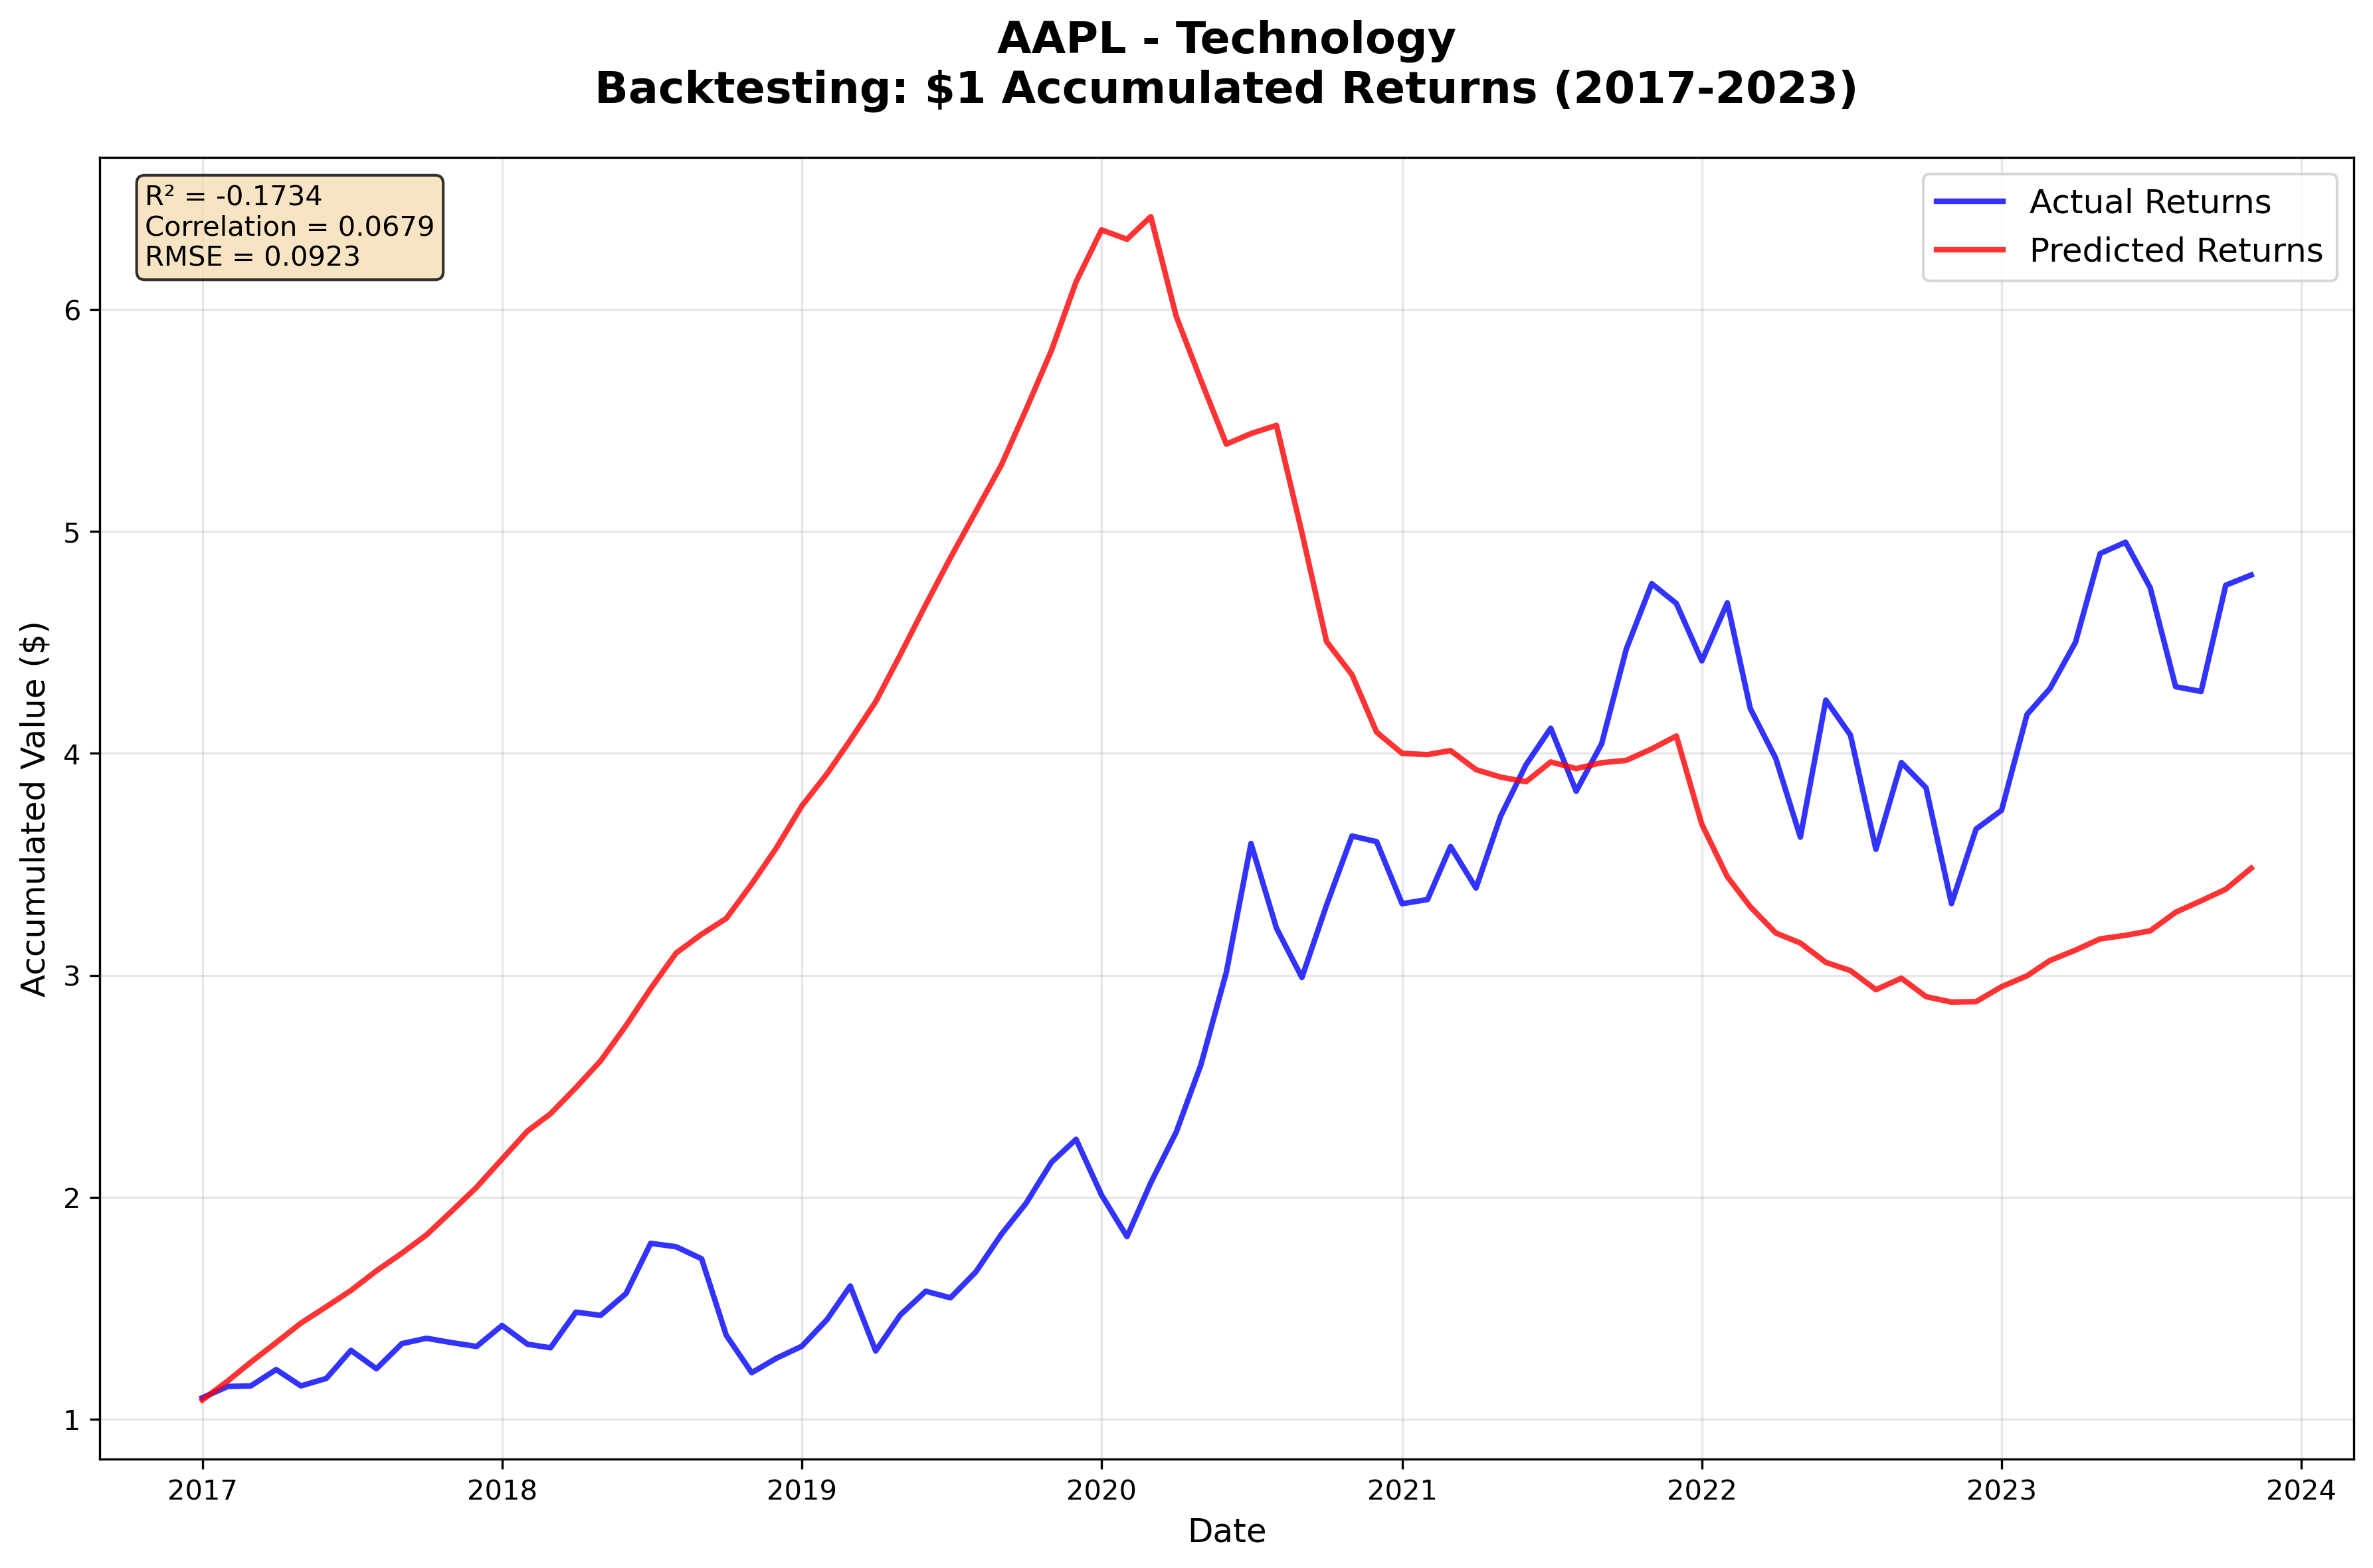
\includegraphics[width=0.31\textwidth]{Plots/AAPL_backtesting.png}}\hfill
    \subfloat[JPM]{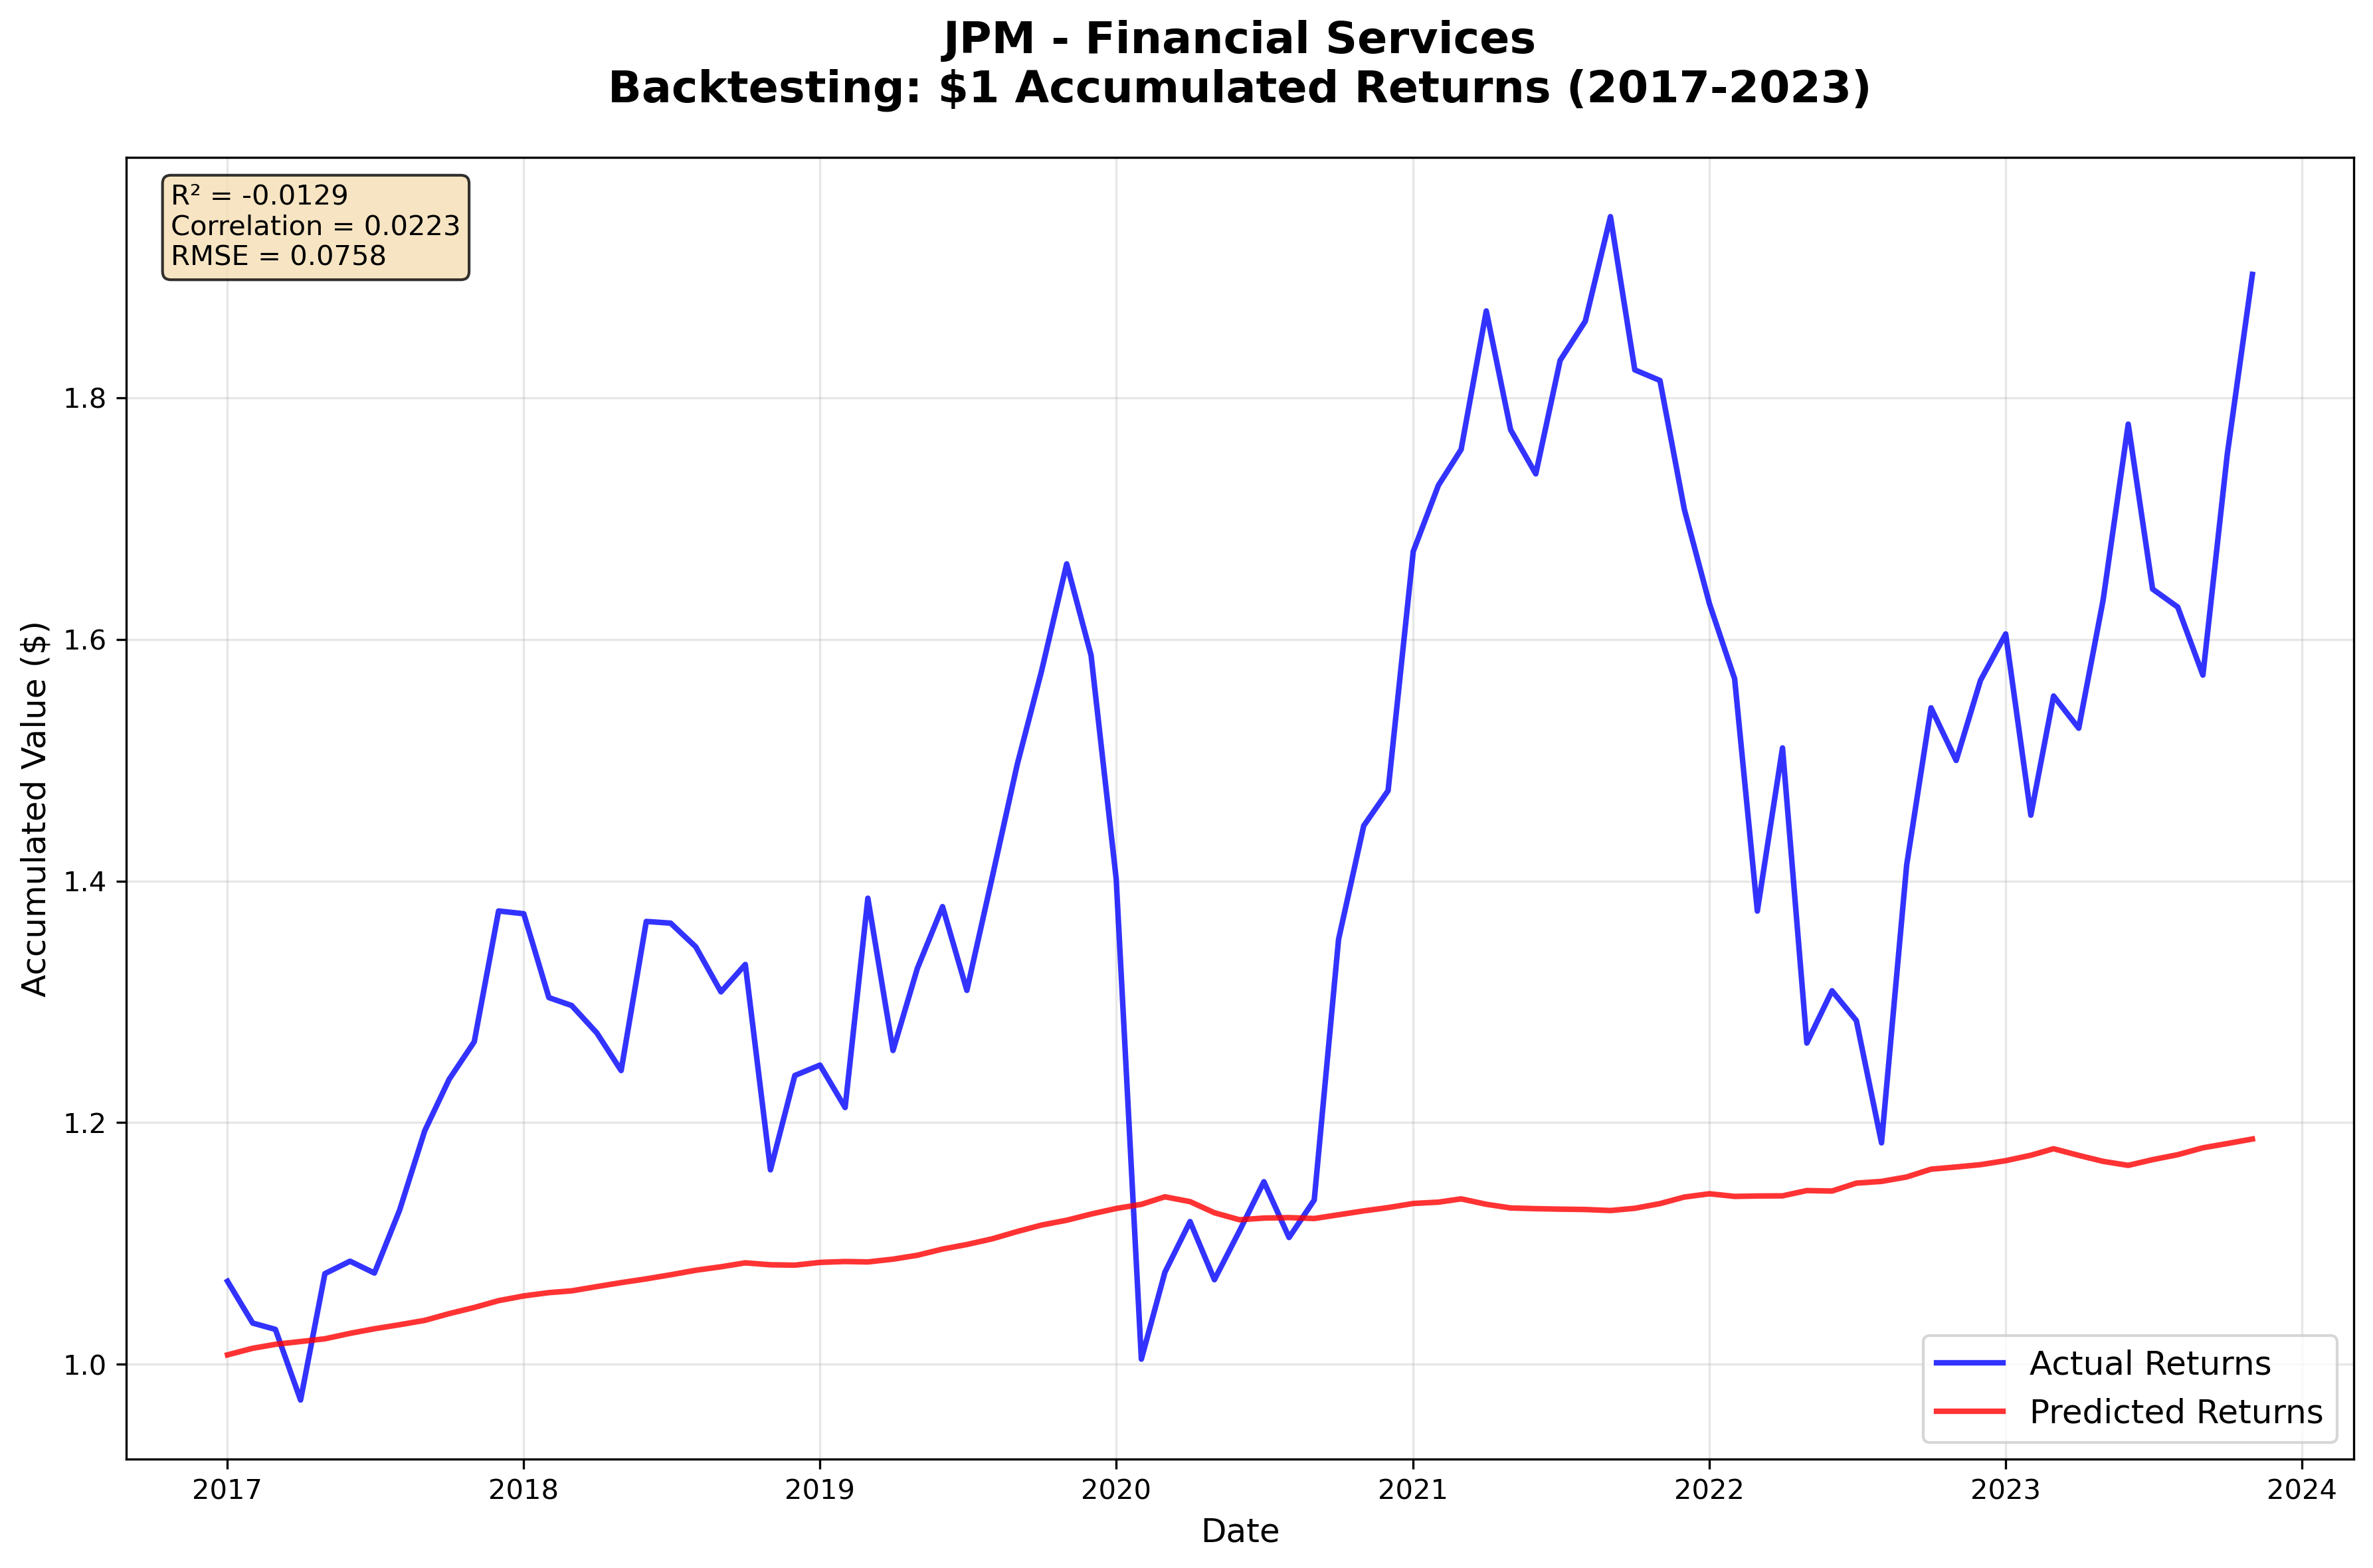
\includegraphics[width=0.31\textwidth]{Plots/JPM_backtesting.png}}\hfill
    \subfloat[JNJ]{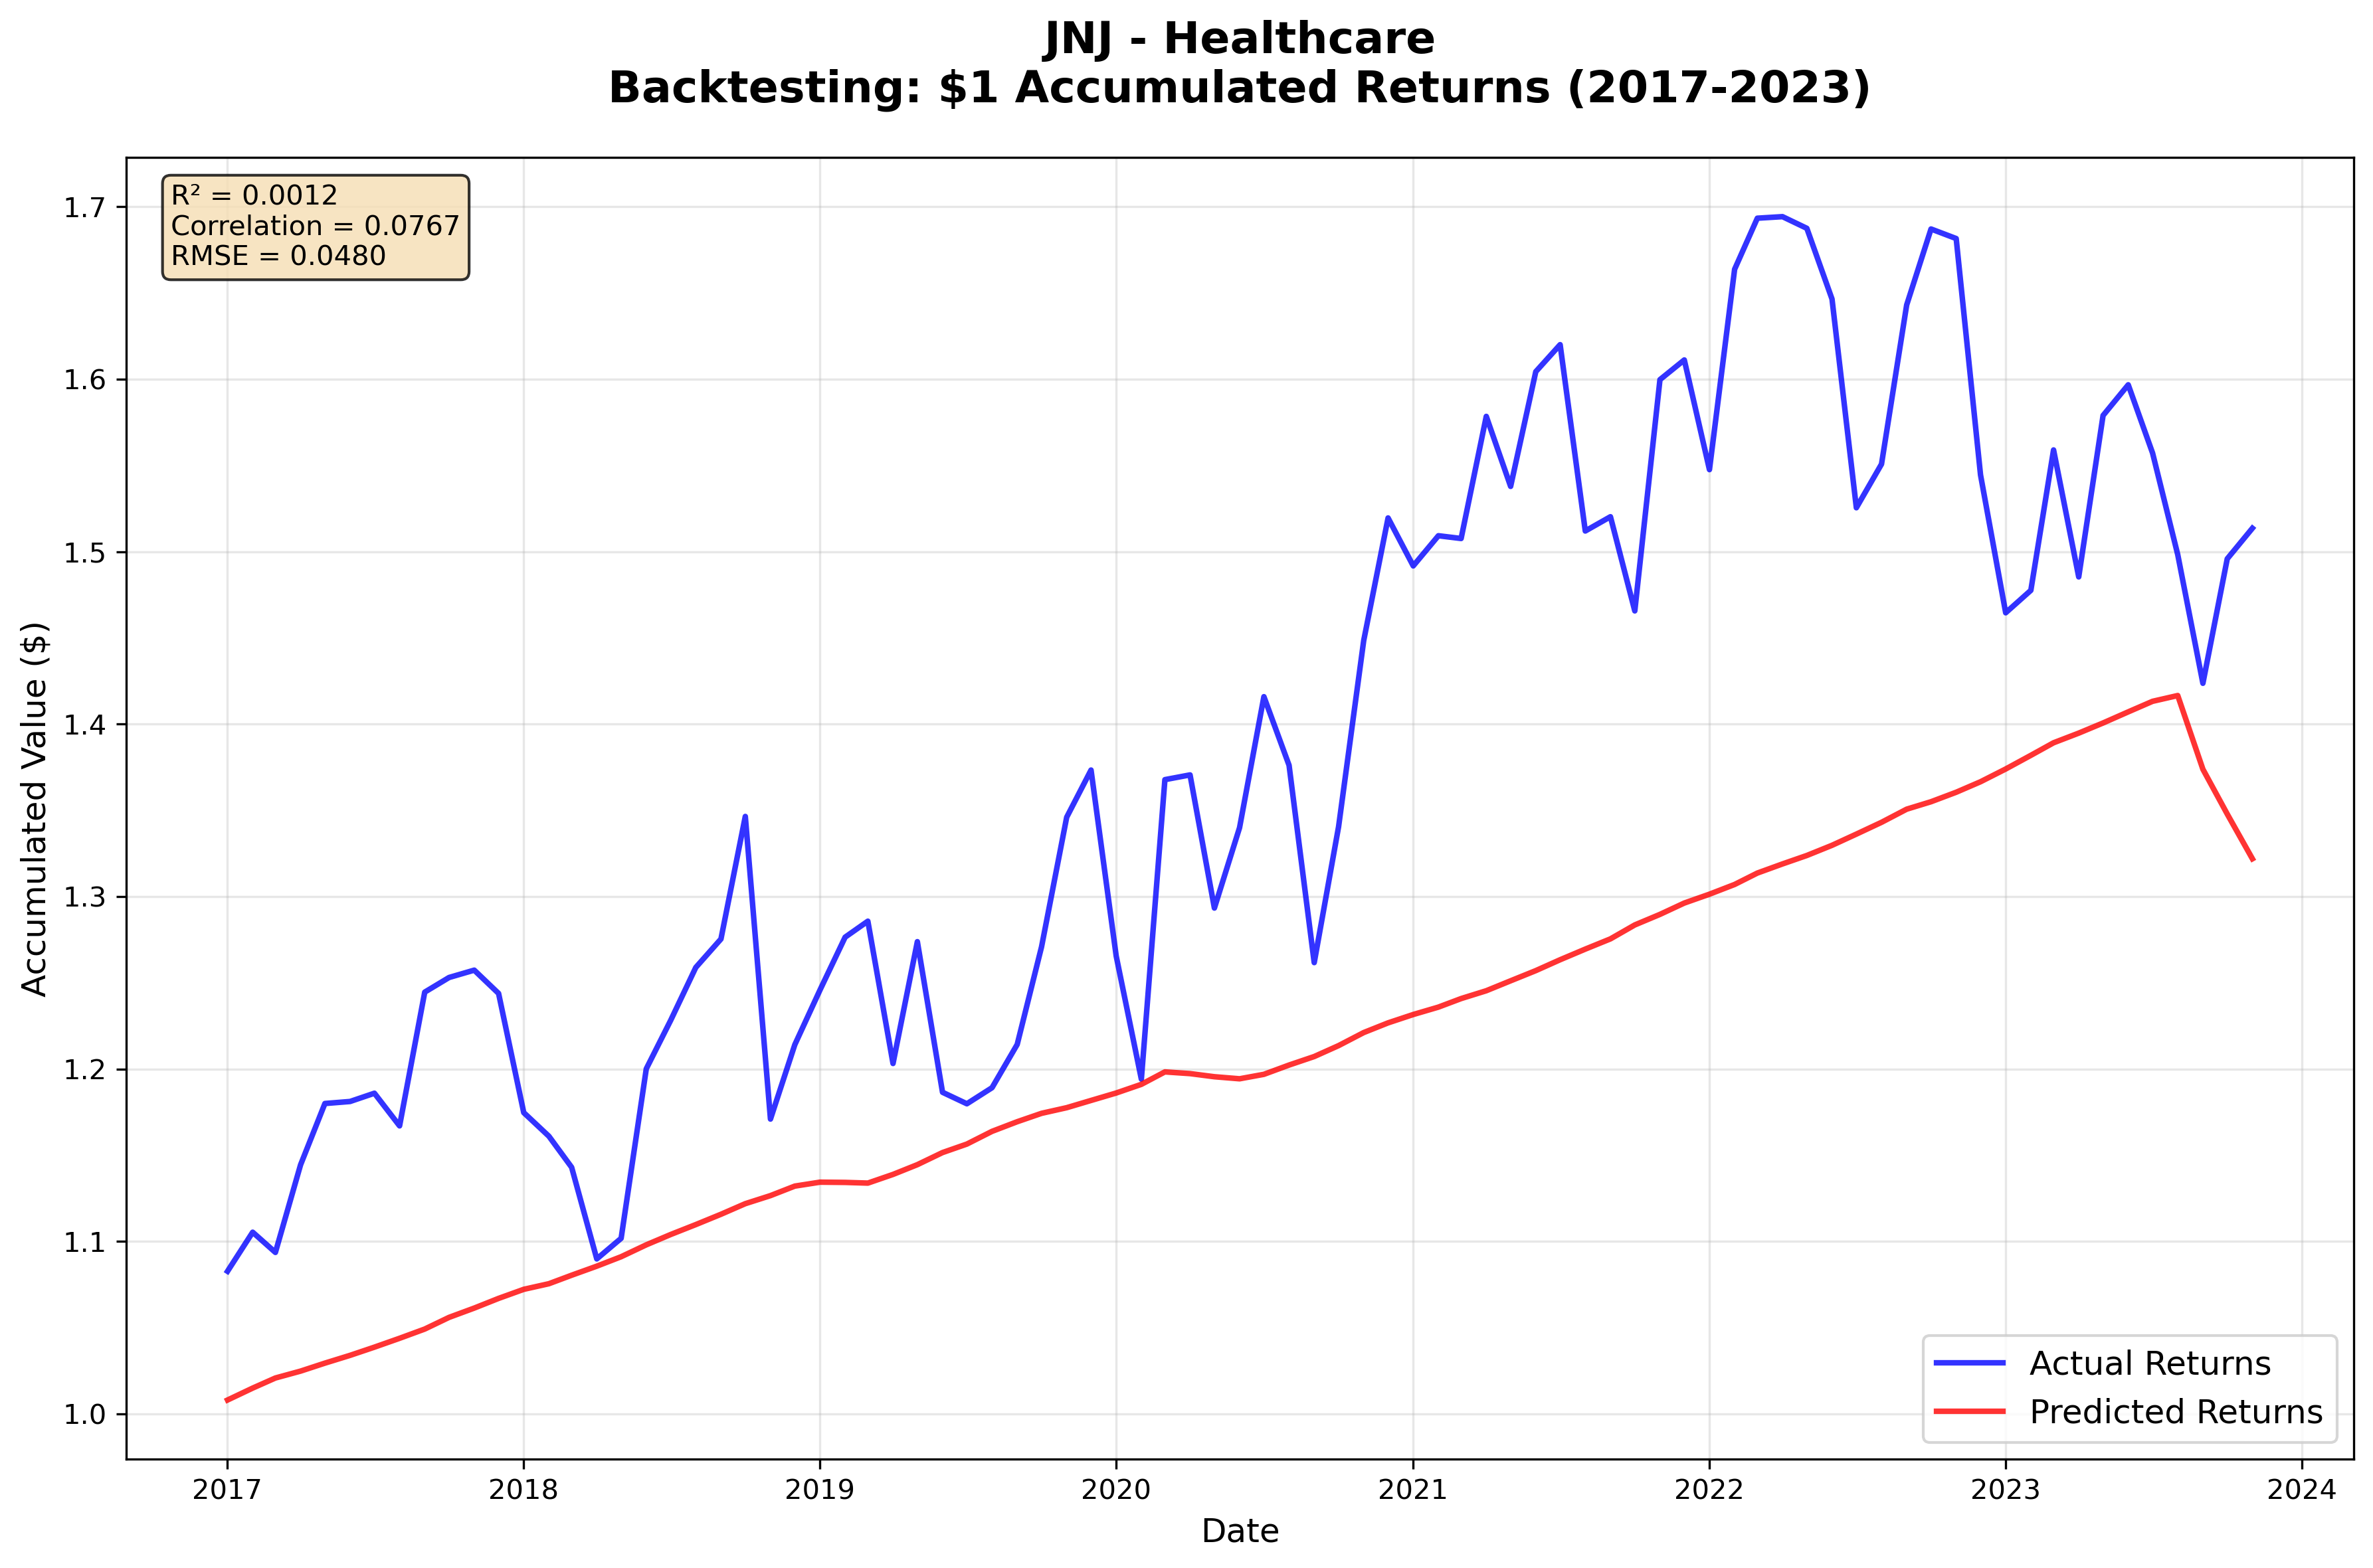
\includegraphics[width=0.31\textwidth]{Plots/JNJ_backtesting.png}}\\[0.4em]
    \subfloat[XOM]{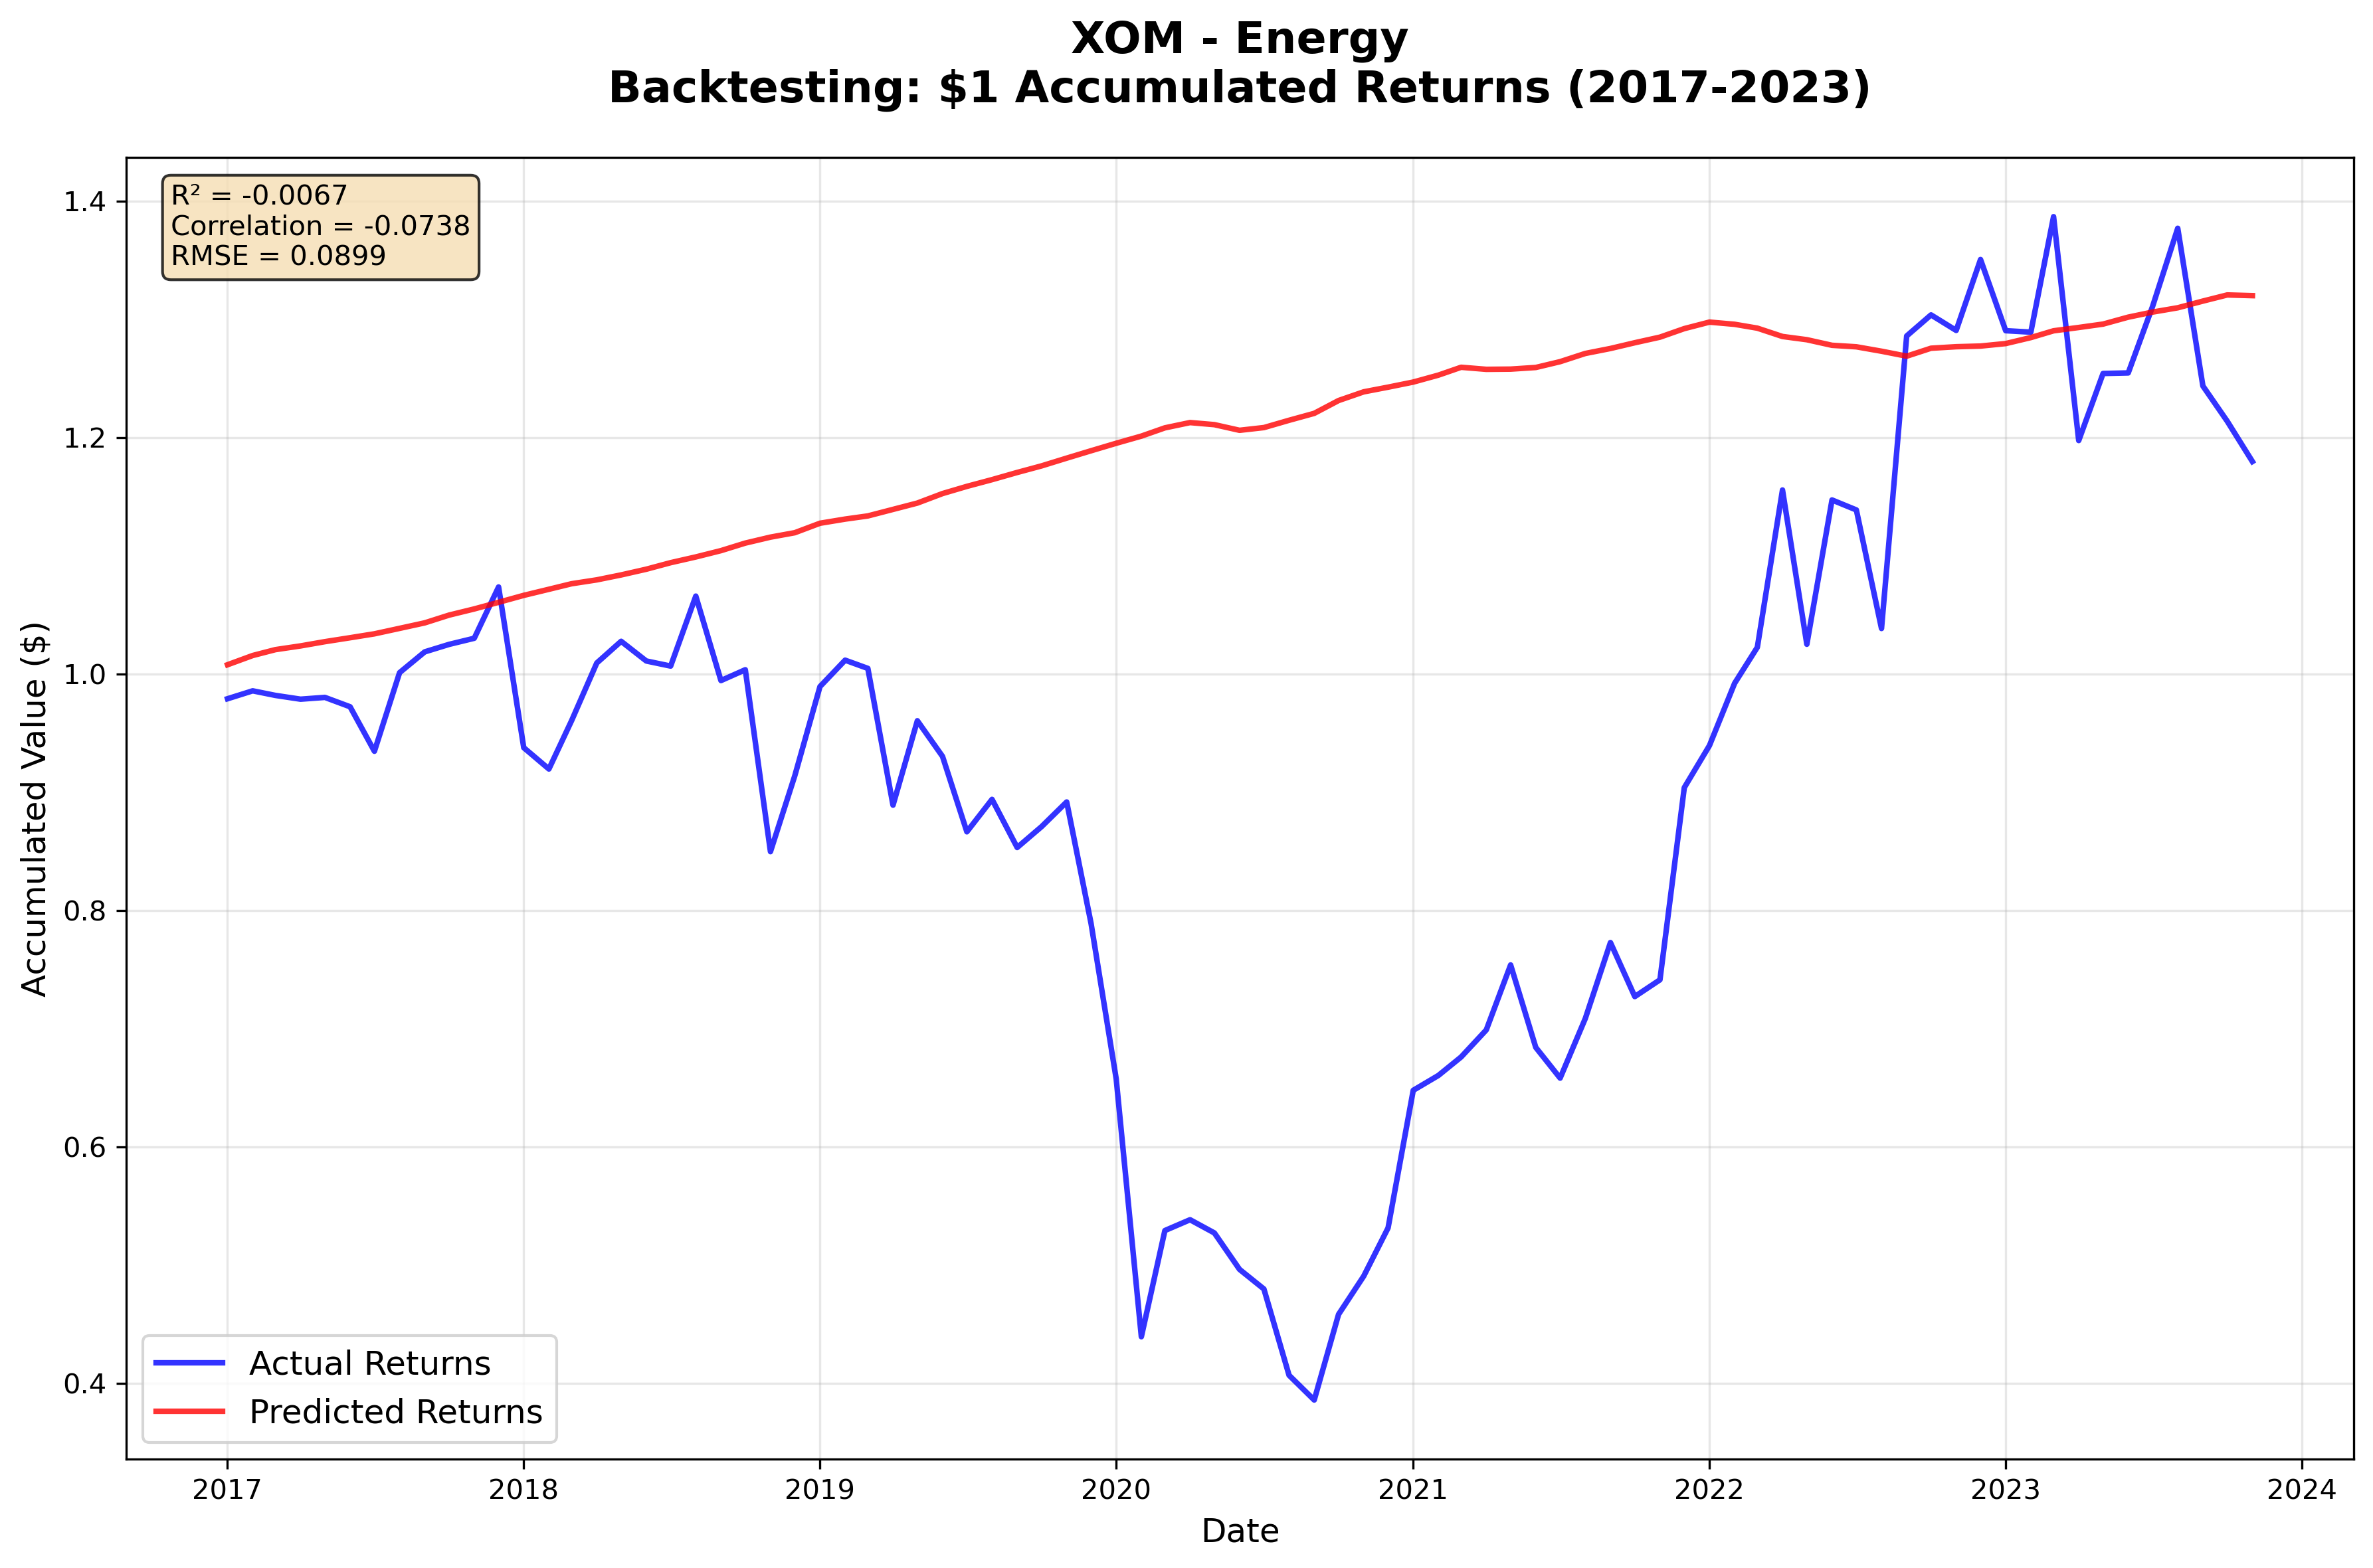
\includegraphics[width=0.31\textwidth]{Plots/XOM_backtesting.png}}\hfill
    \subfloat[AMZN]{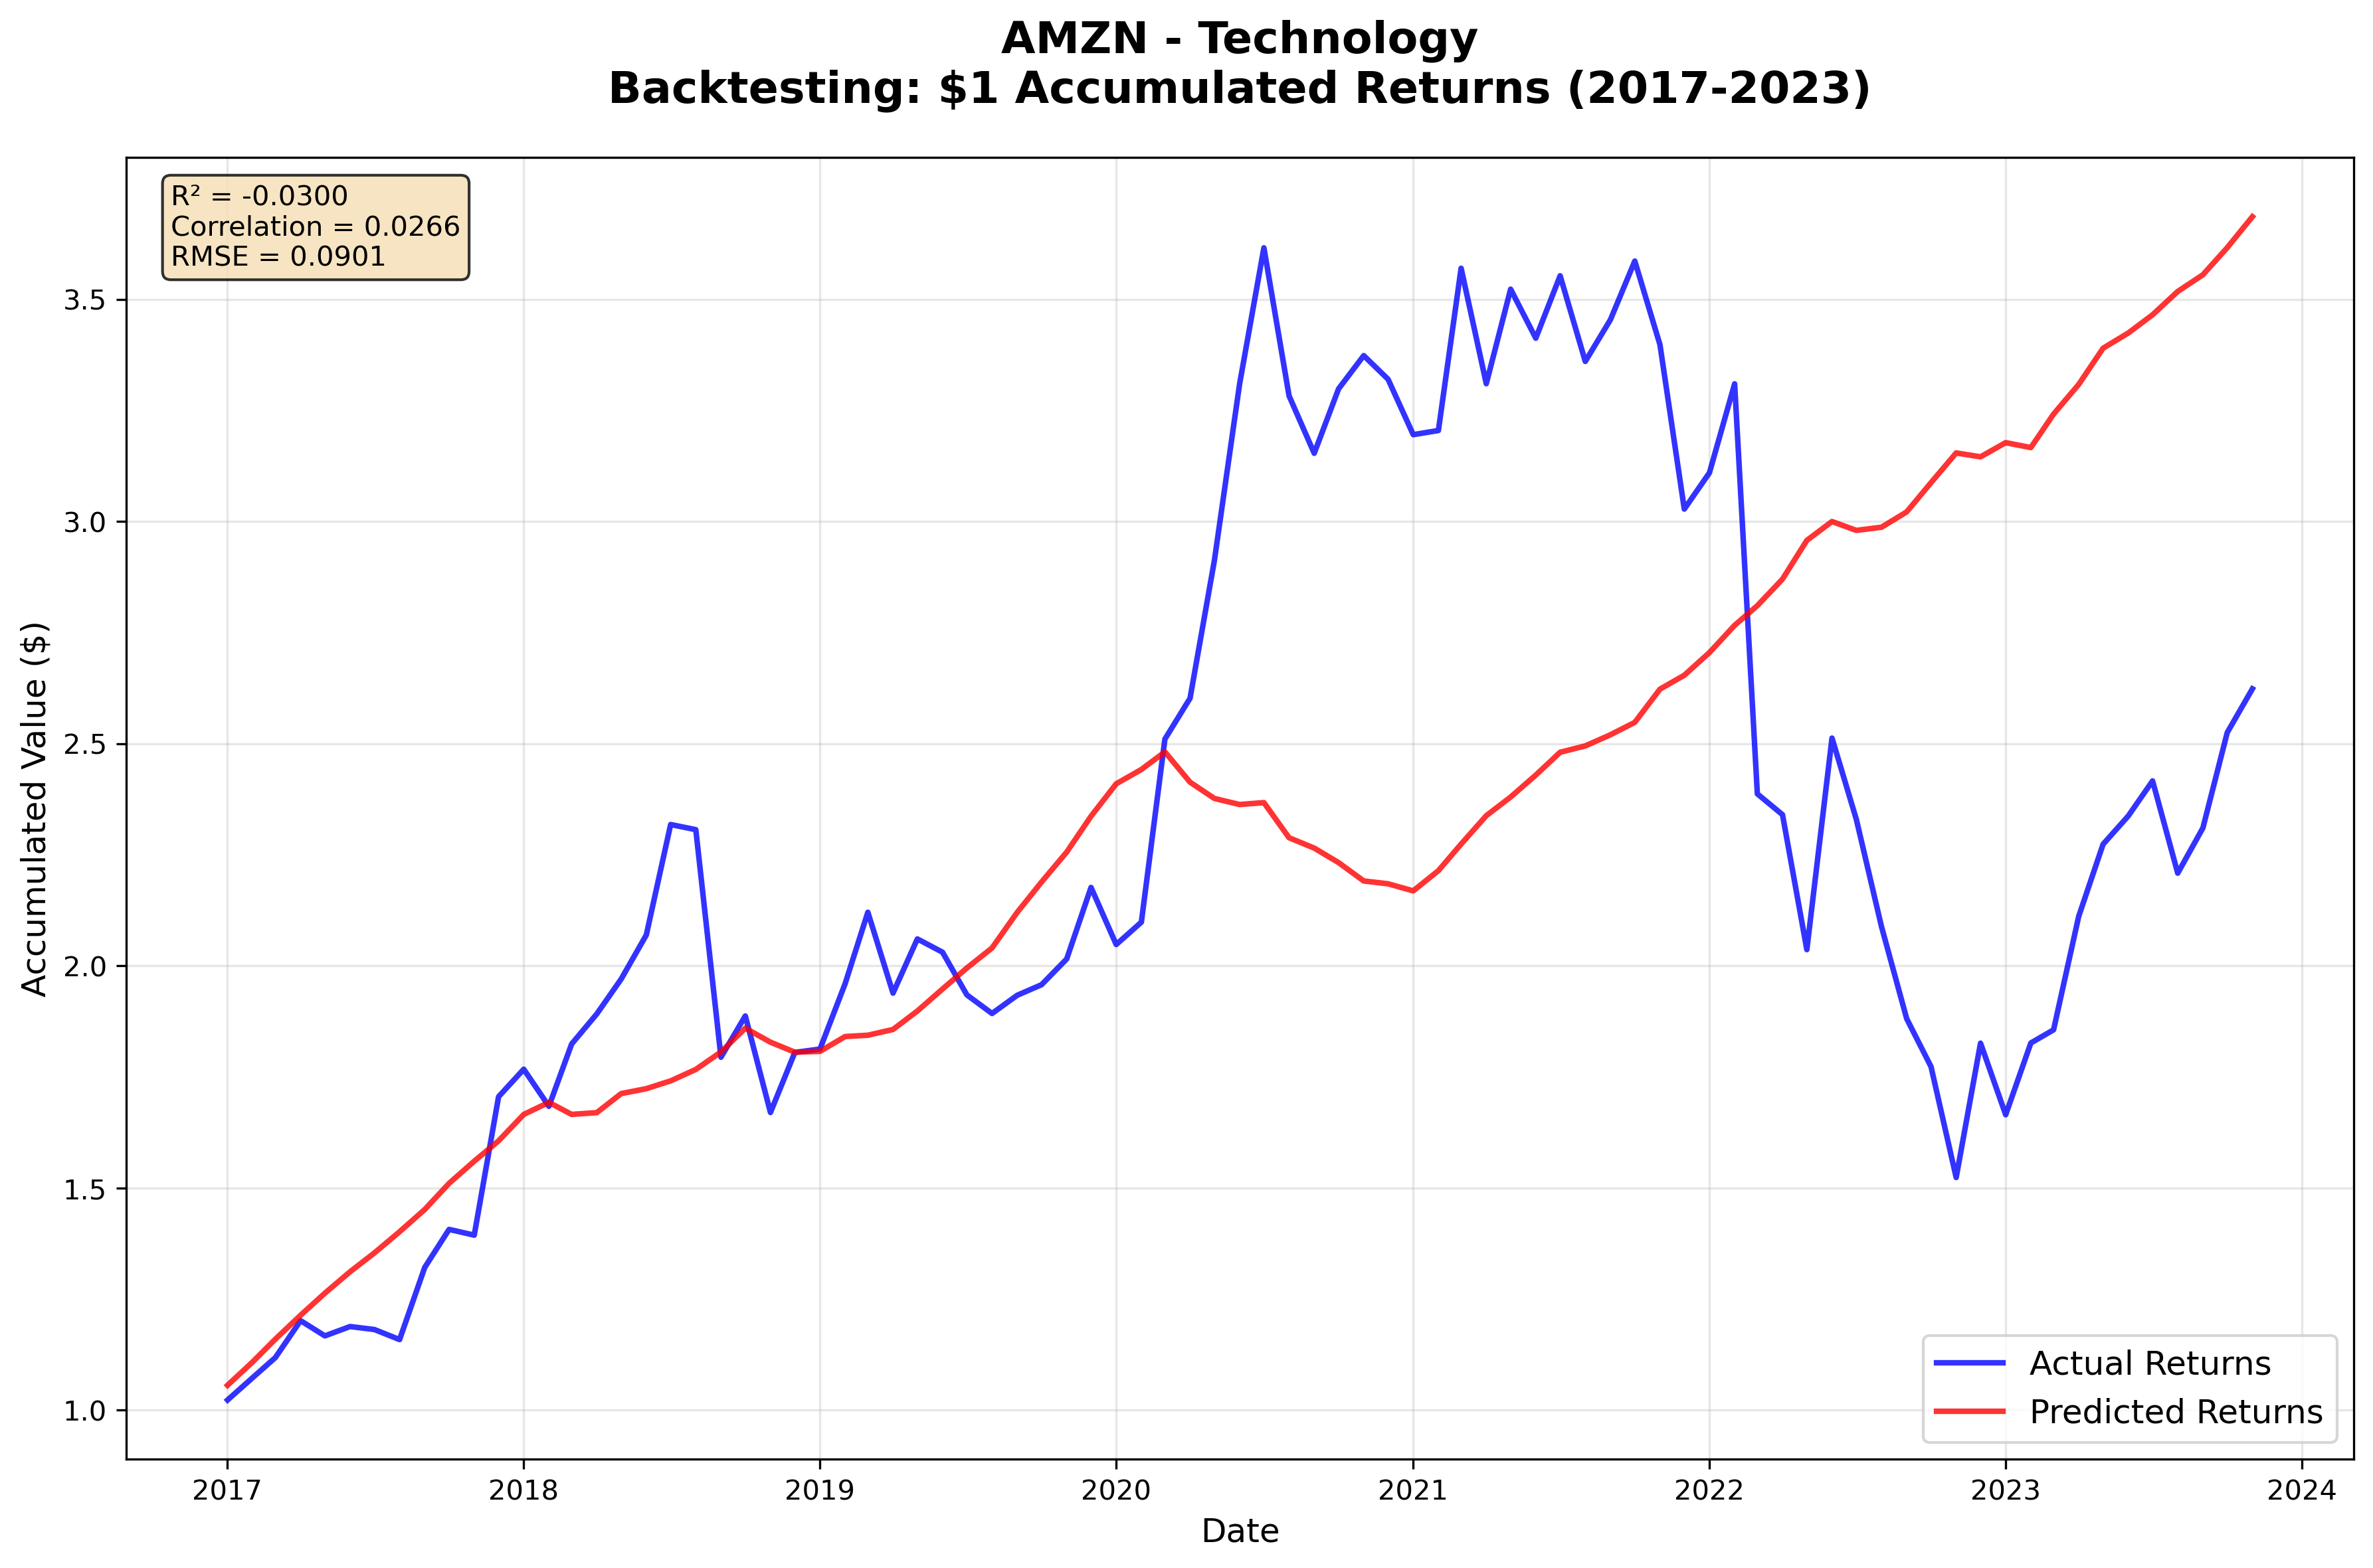
\includegraphics[width=0.31\textwidth]{Plots/AMZN_backtesting.png}}\hfill
    \subfloat[AEP]{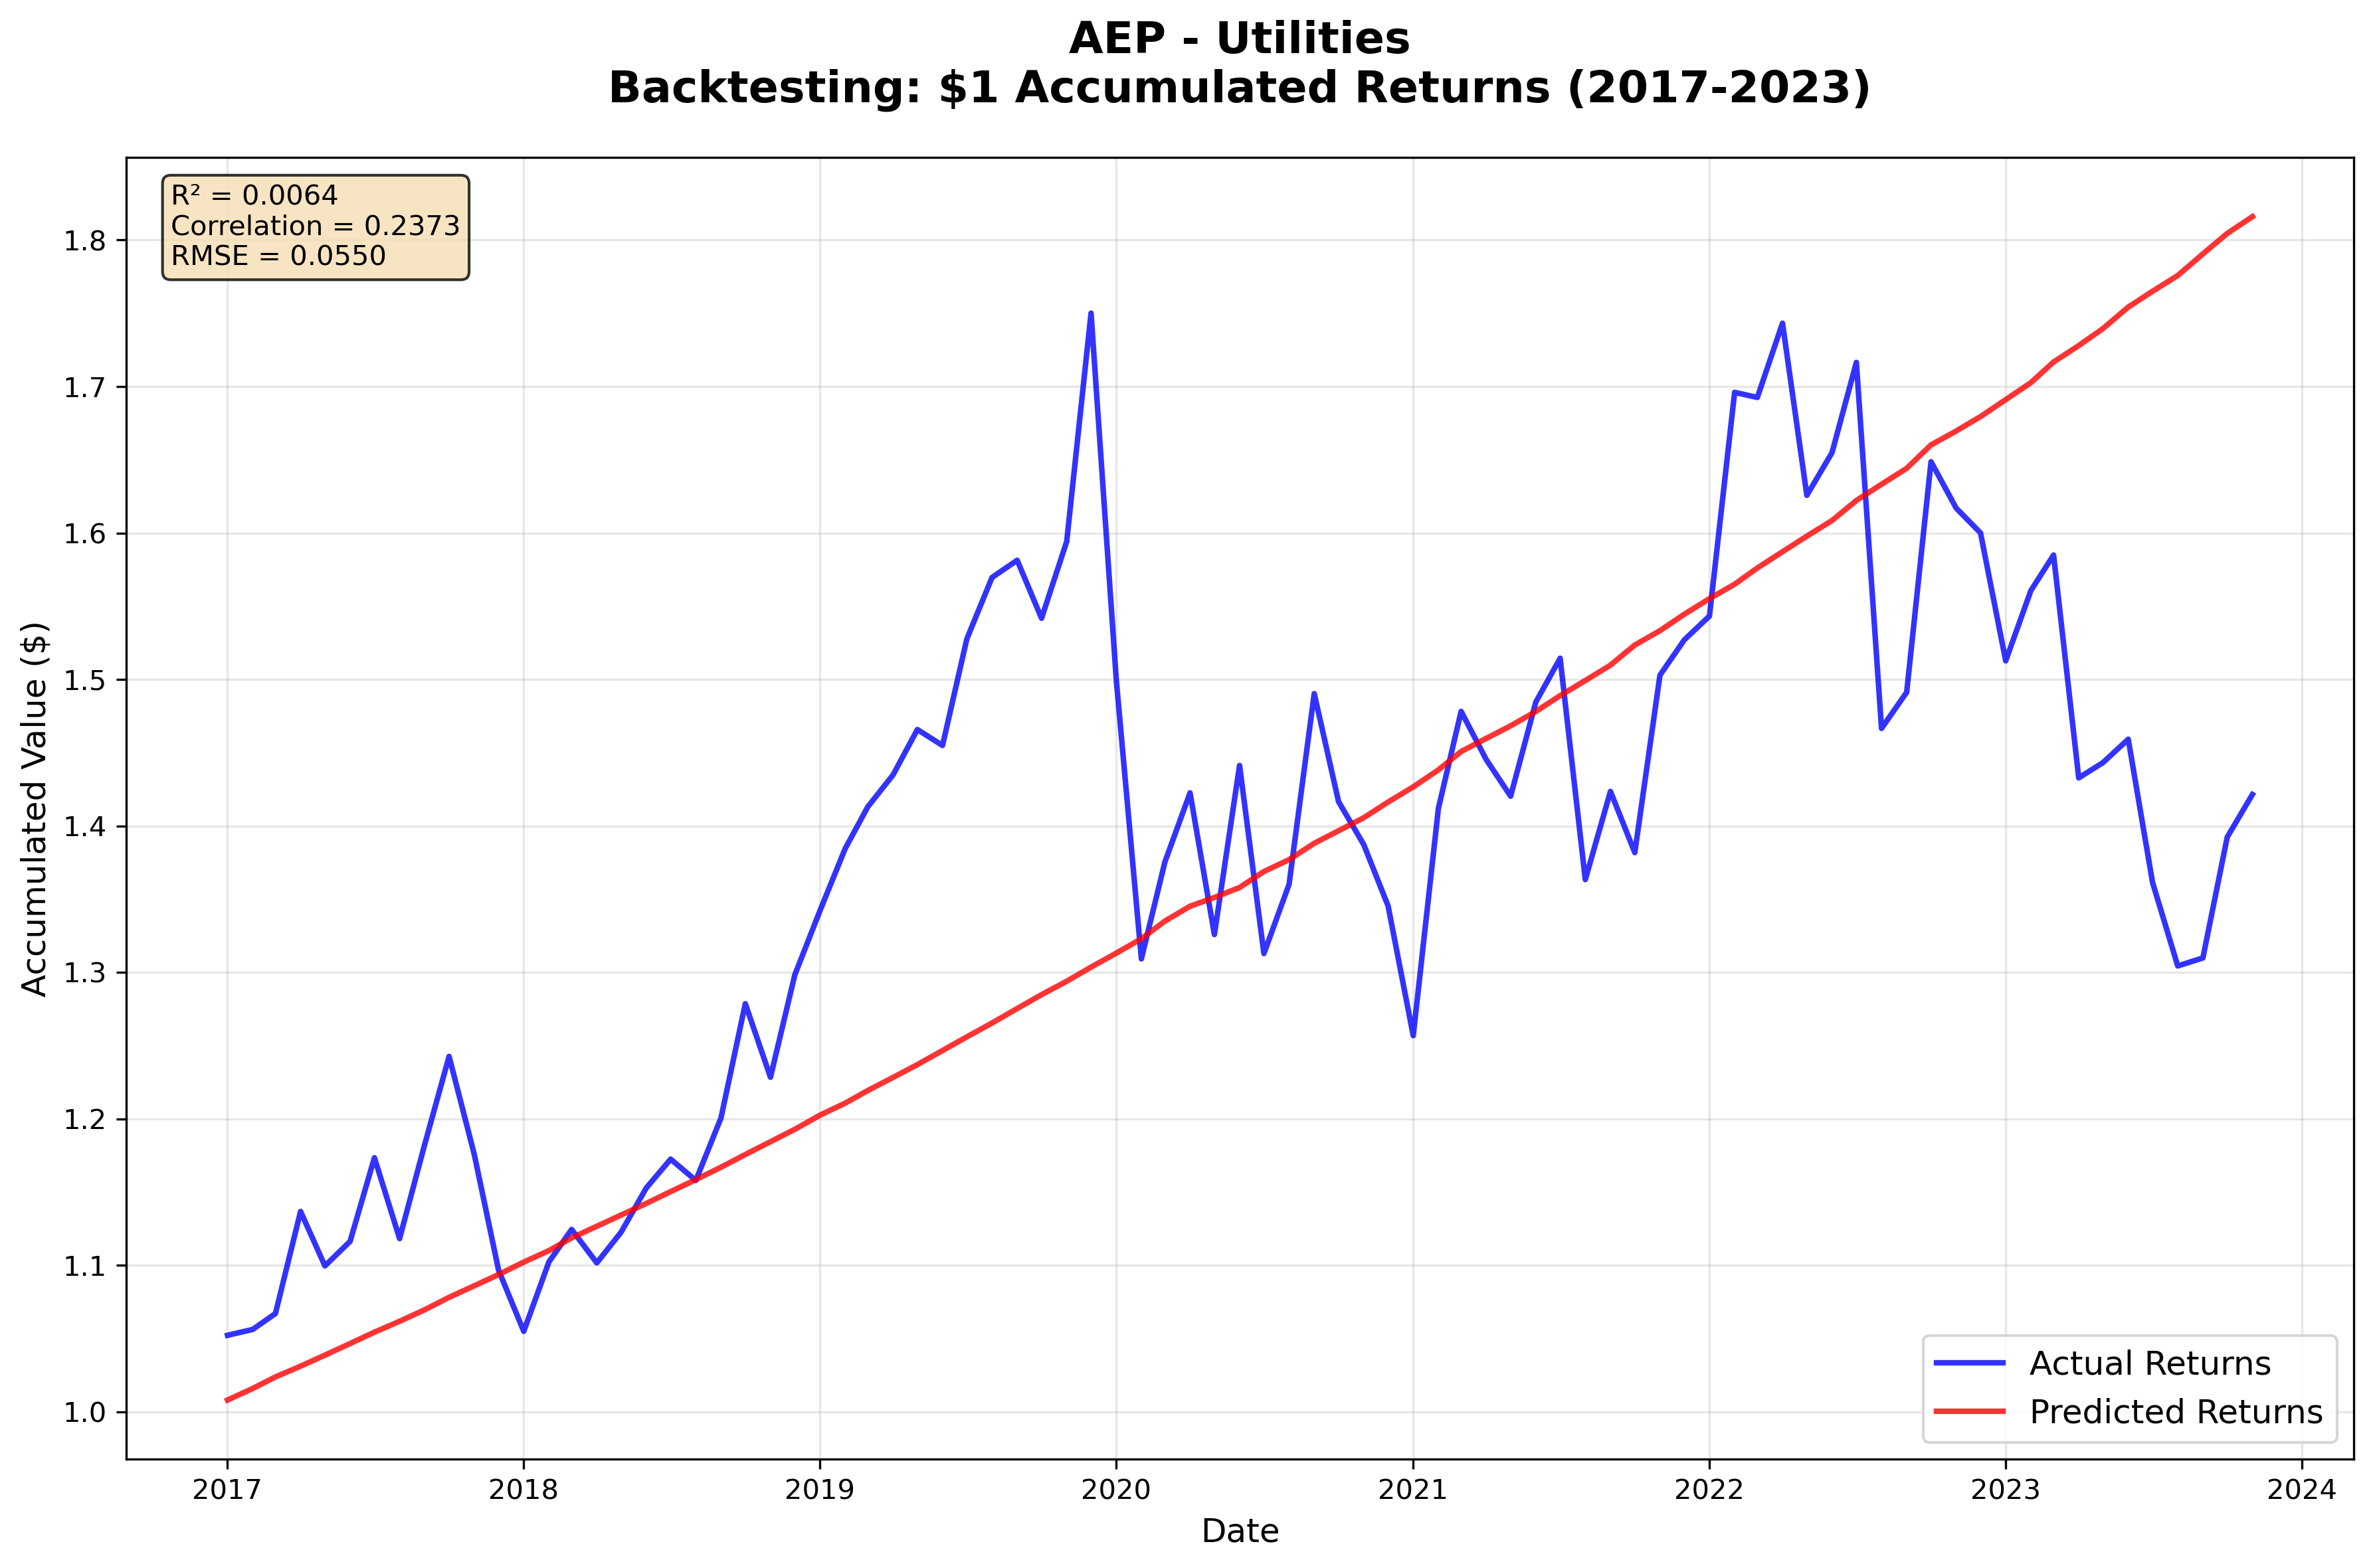
\includegraphics[width=0.31\textwidth]{Plots/AEP_backtesting.png}}
    \caption{\$1 accumulated paths, actual (blue) vs.\ predicted (red), 2017--2023.}
    \label{fig:backtest_plots}
\end{figure*}

Stock-level directional accuracies in the six-name set are 65.1\% (AAPL), 46.9\% (JPM), 56.6\% (JNJ), 55.4\% (XOM), 57.8\% (AMZN), and 62.7\% (AEP). JNJ has a slightly positive stock-level $R^2$ ($0.0012$). Predicted paths are smoother than actual paths: regularization shrinks forecasts toward the intercept, so the model can get the sign of a trend and still miss its size (AAPL actual wealth far exceeds the predicted path).

This is a magnitude-versus-sign gap, not evidence of a tradable edge. No costs, no position caps, and no statistical test that 54.6\% differs from 50\% after multiple names are reported.

\subsection{Discussion}

The 1998--2017 training window includes the dot-com crash and 2008 but not COVID. Negative weights on turnover and volatility match a ``high activity, lower next-month return'' pattern in that sample. In 2020--2021 those same traits often coincided with winners, so a frozen model reads the boom as risk. That is a limitation of set-and-forget coefficients, not a test of every machine learning method.

An intraday (minute-ahead) design---5/30/60-minute momentum, 60-minute beta, and so on---was sketched as future work and is \emph{not} estimated here.

\section{Conclusion}

Minute files for large-cap U.S.\ stocks can be turned into a monthly supervised-learning panel. With 13 constructed predictors, regularized linear models are the only specifications that remain numerically stable, and even those do not produce positive out-of-sample return $R^2$ on 2017--2023. Directional accuracy sits a few points above one-half. The honest reading is that this pipeline is a useful way to learn empirical-asset-pricing machine learning under real data constraints, not a demonstration that high-frequency aggregates unlock monthly alpha.

Code, monthly feature files, coefficients, and plots are provided in the companion repository. Raw minute bars are omitted.

\bibliographystyle{apalike}
\bibliography{references}

\end{document}
